\documentclass[11pt]{book}
\usepackage[utf8]{inputenc}
\usepackage[T1]{fontenc}
\usepackage{amssymb}
\usepackage{tikz}
\usepackage{xcolor}

\begin{document}

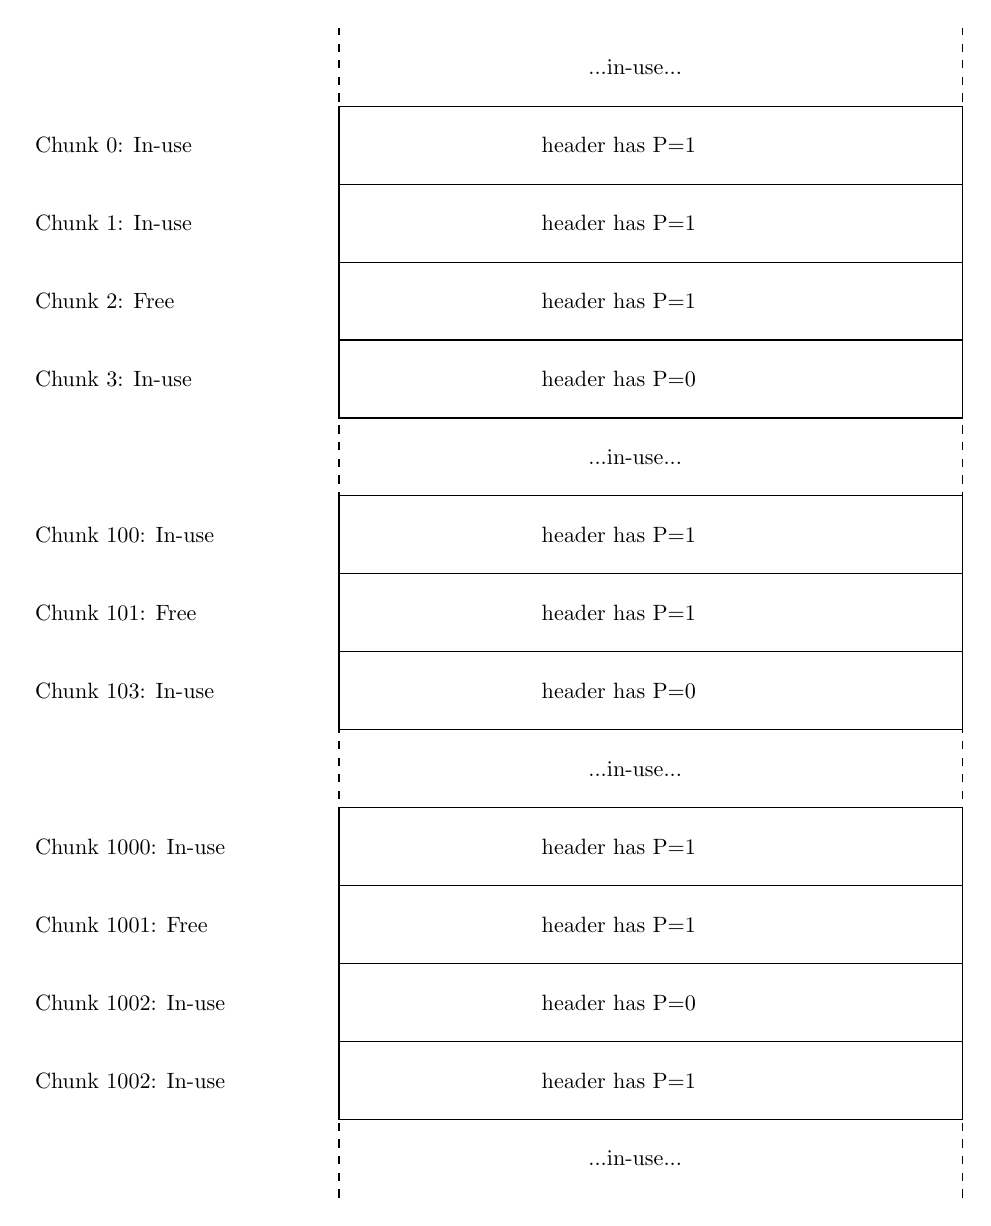
\begin{tikzpicture}[scale=0.99, every node/.style={scale=0.8}]
    % Dotted lines for memory band of 8 byte blocks
    \draw[dashed] (4,0) -- (4,15);
    \draw[dashed] (12,0) -- (12,15);

    % ... Ellipses to represent continuation
    \node[anchor=east] at (8.5,14.5) {...in-use...};

    % Chunk - In-use
    \draw (4,13) rectangle (12,14);
    \node[anchor=west] at (0,13.5) {Chunk 0: In-use};
    \node[anchor=west] at (6.5,13.5) {header has P=1};

    % Chunk - In-use
    \draw (4,12) rectangle (12,13);
    \node[anchor=west] at (0,12.5) {Chunk 1: In-use};
    \node[anchor=west] at (6.5,12.5) {header has P=1};

    % Chunk - Free
    \draw (4,11) rectangle (12,12);
    \node[anchor=west] at (0,11.5) {Chunk 2: Free};
    \node[anchor=west] at (6.5,11.5) {header has P=1};

    % Chunk - In-use
    \draw (4,10) rectangle (12,11);
    \node[anchor=west] at (0,10.5) {Chunk 3: In-use};
    \node[anchor=west] at (6.5,10.5) {header has P=0};

    % Chunks - from top to bottom (inverted order)
    % ... Ellipses to represent continuation
    \node[anchor=east] at (8.5,9.5) {...in-use...};

    % Chunk - In-use
    \draw (4,8) rectangle (12,9);
    \node[anchor=west] at (0,8.5) {Chunk 100: In-use};
    \node[anchor=west] at (6.5,8.5) {header has P=1};

    % Chunk - Free
    \draw (4,7) rectangle (12,8);
    \node[anchor=west] at (0,7.5) {Chunk 101: Free};
    \node[anchor=west] at (6.5,7.5) {header has P=1};

    % Chunk - In-use, P=0
    \draw (4,6) rectangle (12,7);
    \node[anchor=west] at (0,6.5) {Chunk 103: In-use};
    \node[anchor=west] at (6.5,6.5) {header has P=0};

    % ... Ellipses to represent continuation
    \node[anchor=east] at (8.5,5.5) {...in-use...};

    % Chunk - In-use
    \draw (4,4) rectangle (12,5);
    \node[anchor=west] at (0,4.5) {Chunk 1000: In-use};
    \node[anchor=west] at (6.5,4.5) {header has P=1};

    % Chunk - Free
    \draw (4,3) rectangle (12,4);
    \node[anchor=west] at (0,3.5) {Chunk 1001: Free};
    \node[anchor=west] at (6.5,3.5) {header has P=1};

    % Chunk - In-use, P=0
    \draw (4,2) rectangle (12,3);
    \node[anchor=west] at (0,2.5) {Chunk 1002: In-use};
    \node[anchor=west] at (6.5,2.5) {header has P=0};

    % Chunk - In-use,
    \draw (4,1) rectangle (12,2);
    \node[anchor=west] at (0,1.5) {Chunk 1002: In-use};
    \node[anchor=west] at (6.5,1.5) {header has P=1};

    % ... Ellipses to represent continuation
    \node[anchor=east] at (8.5,0.5) {...in-use...};

\end{tikzpicture}

\end{document}